\documentclass[14pt]{article}

%\documentclass[fleqn]{article}
%\usepackage{palatino} 
%\usepackage{charter}
%\usepackage[T1]{fontenc}
%\usepackage{concmath} % pretty good
%\usepackage{cmbright}
%%%%%%%%%%%%%%%%%%%%%%%%%%%%%%%%%%%%%
\usepackage{/home/sci/weiliu/haldefs}
\usepackage{/home/sci/weiliu/notes}
\usepackage{/home/sci/weiliu/projects/lwdefs}
\usepackage{graphicx}
\usepackage{url}
\usepackage{textcomp}
%\usepackage[numbers]{natbib}
\usepackage{natbib}
%\usepackage{subfig}
\usepackage{hyperref}
\usepackage{/home/sci/weiliu/packages/breakurl/breakurl}
%\usepackage{endfloat}
\usepackage{amsmath}
\usepackage{verbatim}
\usepackage{algorithmic}
\usepackage{algorithm}
\usepackage{html}

\hypersetup{
    bookmarks=true,         % show bookmarks bar?
    unicode=false,          % non-Latin characters in Acrobat’s bookmarks
    pdftoolbar=true,        % show Acrobat’s toolbar?
    pdfmenubar=true,        % show Acrobat’s menu?
    pdffitwindow=false,     % window fit to page when opened
    pdfstartview={FitH},    % fits the width of the page to the window
    pdftitle={Scale-Space Blob Detection},    % title
    pdfauthor={Wei Liu},     % author
    pdfsubject={Project for advanced Image Processing},   % subject of the document
    pdfcreator={Wei Liu},   % creator of the document
    pdfproducer={Producer}, % producer of the document
    pdfkeywords={blob detection, scale-space}, % list of keywords
    pdfnewwindow=true,      % links in new window
    colorlinks= true,       % false: boxed links; true: colored links
    linkcolor=red,          % color of internal links
    citecolor=green,        % color of links to bibliography
    filecolor=magenta,      % color of file links
    urlcolor=cyan           % color of external links
}



\begin{document}
\title{Markov Random Field and application on fMRI Connectivity Analysis}
\author{Wei Liu\\ weiliu@sci.utah.edu}
\maketitle
\tableofcontents
\textbf{Goal: } Compute the 'connectivity' between any pair of voxels (or regions) in brain cortex. (the rigid definition of 'connectivity' is not available.)

\textbf{information available: }
\begin{itemize}
\item Data. fMRI (time courses), DTI(tractography)
\item Assumption: Connectivity should be smoothly changed.
\end{itemize}
\textbf{Method: } Bayesian Rule:
\begin{equation}
p(\mbox{connectivity})\propto prior(\mbox{connectivity}) \cdot \mbox{likelihood}
\end{equation}

\textbf{Prior: } 1) from neighbors connectivity. 2) from other voxels with DTI tract.
\textbf{likelihood: } from data.

1) From neighbors connectivity. 
\begin{figure}[htb]
\centering
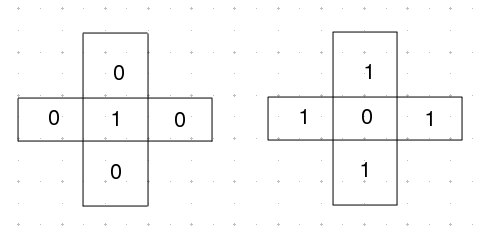
\includegraphics[width = 0.8\textwidth]{mrf1.png}
\caption{Without data, the connectivity value at a point depends on its neighbors.}
\label{fig1}
\end{figure}

\begin{figure}[htb]
\centering
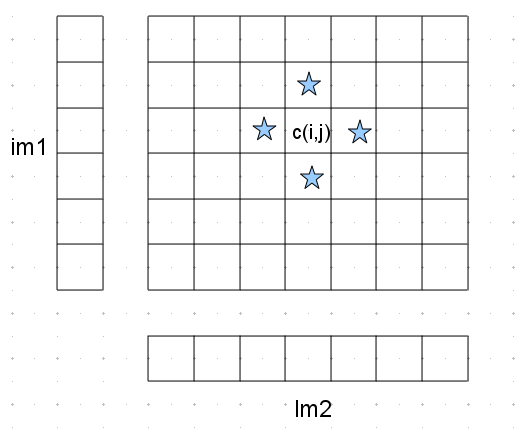
\includegraphics[width = 0.8\textwidth]{1d.png}
\caption{Connectivity between any voxel pairs of two 1-D image. }
\label{fig2}
\end{figure}

\begin{figure}[htb]
\centering
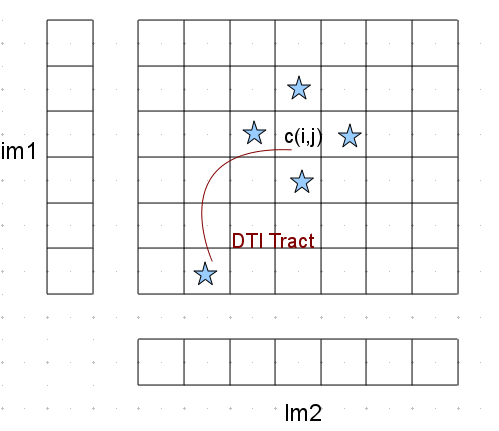
\includegraphics[width = 0.8\textwidth]{dti.png}
\caption{Connectivity between any voxel pairs of two 1-D image, with DTI tract. }
\label{fig3}
\end{figure}
\begin{figure}[htb]
\centering
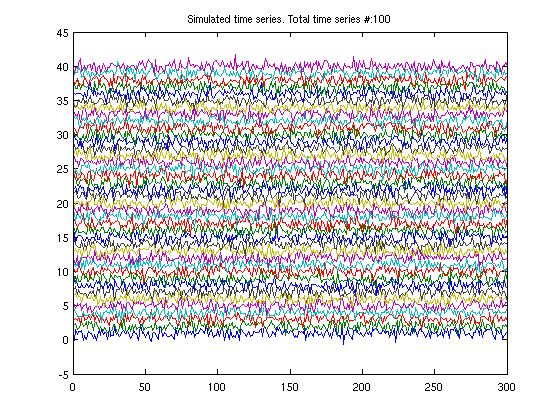
\includegraphics[width = 0.5\textwidth]{sin.png}
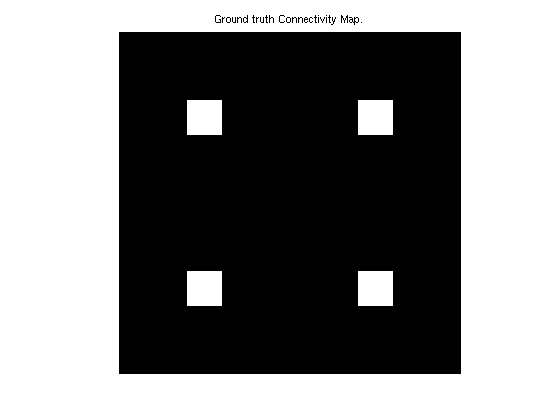
\includegraphics[width = 0.5\textwidth]{true.png}
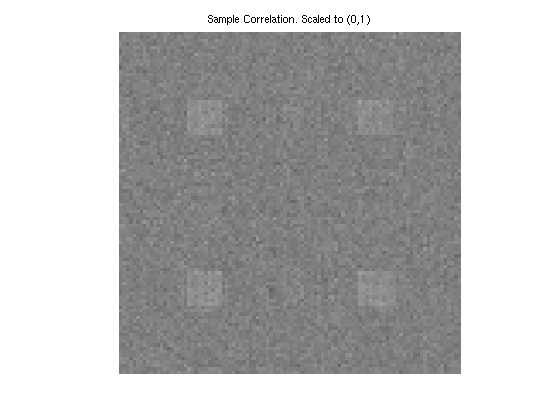
\includegraphics[width = 0.8\textwidth]{correlation.png}
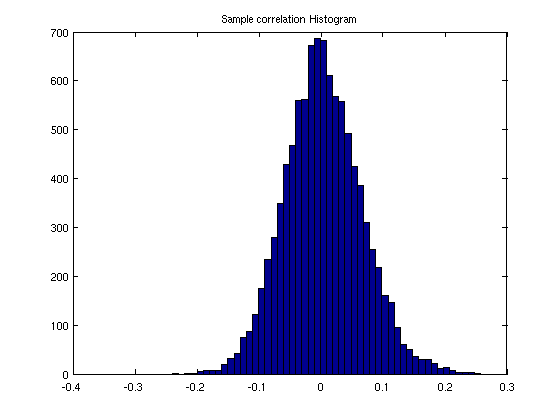
\includegraphics[width = 0.8\textwidth]{hist.png}
\caption{synthetic image}
\label{fig4}
\end{figure}

\begin{figure}[htb]
\centering
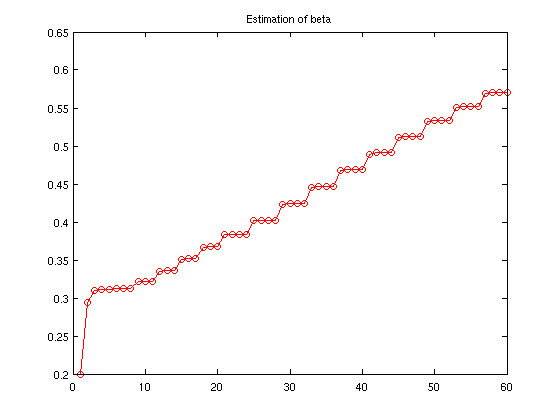
\includegraphics[width = 0.5\textwidth]{../results/beta.png}
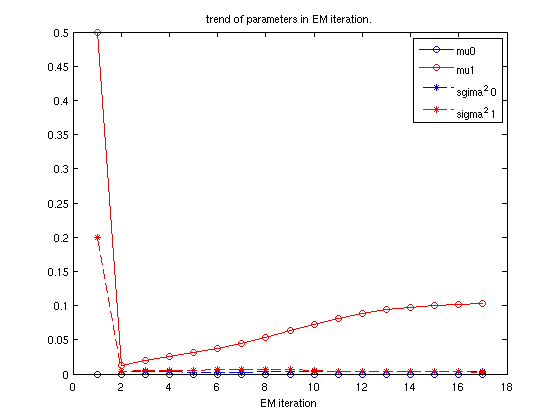
\includegraphics[width = 0.5\textwidth]{../results/para_est.png}

\includegraphics[width = 0.5\textwidth]{../results/postP1.png}
\caption{Use Markov Random Field to estimate connectivity.}
\label{fig5}
\end{figure}

A dynamic plot can be found here: \url{http://www.sci.utah.edu/~weiliu/research/intro/postConn.gif}

\textbf{What questions can we answer: }
\begin{itemize}
\item Build resting state brain network?\cite{hayasaka_comparison_2010}
\item find similar connectivity among groups?\cite{schn_similar_???}
\item causality?
\end{itemize}


\bibliographystyle{plainnat}
\bibliography{/home/sci/weiliu/projects/zotero}
\end{document}
